\section{Methodology}

\subsection{Data Preprocessing}

Using the analysis and data exploration above, we've built the following preprocessing pipeline (the same cleaning process will also be applied on the training and testing datasets):

\begin{figure}[h]
\centering
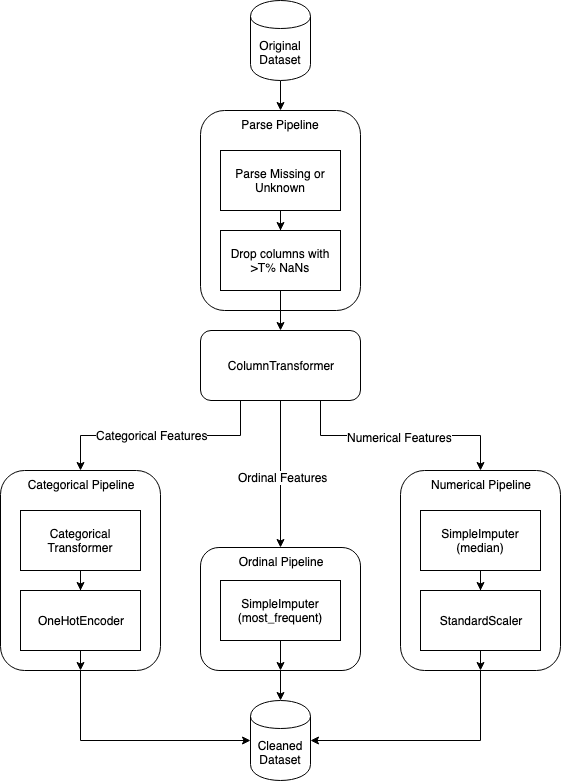
\includegraphics[width=0.5\textwidth]{preprocessing_pipeline.png}
\caption{Preprocessing Pipeline}
\label{fig:preprocessing_pipeline}
\end{figure}

The preprocessing pipeline has the following components:

\textbf{Parse pipeline} composed of two steps:
\begin{itemize}
    \item \emph{Parse Missing or Unknown} - custom pipeline that uses the feature summary constructed dataset (column missing\_or \_unknown) to recode values as NaNs.
    \item \emph{Drop columns with T\% NaNs} - Custom pipeline that drops all features that have more than T\% (75\% in our case) missing values
\end{itemize}

\textbf{Column Transform Pipeline} uses the \emph{ColumnTransform} pipeline from sci-kit learn to combine the following pipelines:
\begin{itemize}
    \item \textbf{Categorical Pipeline} applies the following steps to all categorical features:
        \begin{itemize}
            \item \emph{Categorical Transformer} - Custom pipeline transformer (see the paragraph: "Categorical Transformer: below for more details).
            \item \emph{OneHotEncoder} - Encode categorical integer features as a one-hot numeric array.
        \end{itemize}
    \item \textbf{Oridnal Pipeline} applies the following steps to all ordinal features:
        \begin{itemize}
            \item \emph{SimpleImputer} - Imputation transformer for completing missing values by using the most frequent value along each column.
        \end{itemize}
    \item \textbf{Numerical Pipeline} applies the following steps to all numeric features:
        \begin{itemize}
            \item \emph{SimpleImputer} - Imputation transformer for completing missing values by using the mean along each column.
            \item \emph{StandardScaler} - Standardize features by removing the mean and scaling to unit variance
        \end{itemize}        
\end{itemize}

\paragraph{Categorical Transformer}Is a custom pipeline transformer that processes the categorical and mixed-type features by applying the following steps:
\begin{itemize}
    \item Fill in the missing values using the most frequent value along each column
    \item Re-engineer the \emph{PRAEGENDE\_JUGENDJAHRE} mixed-type feature into two additional categorical features \emph{DECADE} and \emph{MOVEMENT} and then drop the original column
    \item Re-engineer the \emph{CAMEO\_INTL\_2015} mixed-type feature into two additional categorical features \emph{WEALTH} and \emph{LIFE\_STAGE} and then drop the original column
\end{itemize}

In figure \ref{fig:features_per_type}, we can see the distribution of feature types before and after dropping features with more than 75\% missing values.

\begin{figure}[h]
\centering
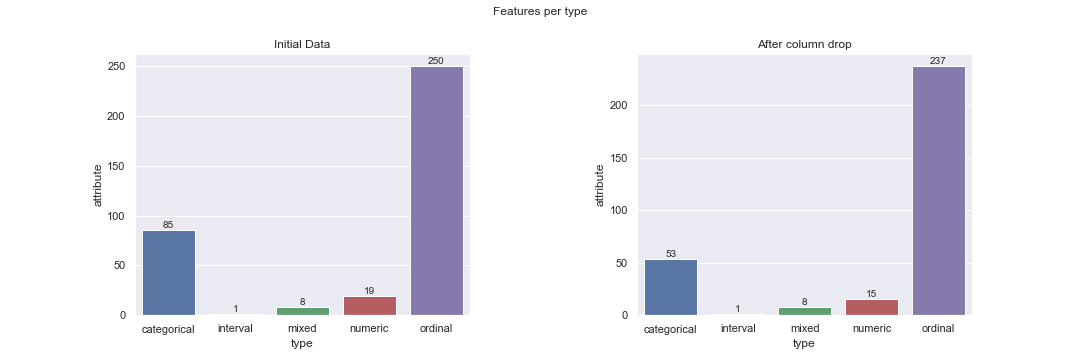
\includegraphics[width=1.0\textwidth]{features_per_type.png}
\caption{Feature per type}
\label{fig:features_per_type}
\end{figure}

We also perform an analysis for rows with a lot of missing values. As we can see in Figure \ref{fig:row_nans}, there are some rows with more than 85\% missing values per row.

To know what to do with the outlier rows, we look the distribution of data values in columns that are not missing data (or are missing very little data) are similar or different between the two groups.

 As we can see in Figure \ref{fig:row_distributions} in Section \ref{ANNEX}, the data with many missing values looks very different from the data with few or no missing values. We decide not to remove these rows.

\subsection{Implementation}

\subsubsection{Perform Dimensionality Reduction}

On our preprocessed data, we are now ready to apply dimensionality reduction techniques.

We use sklearn's PCA class to apply principal component analysis on the data, thus finding the vectors of maximal variance in the data. 

We start by fitting a PCA on 685 dimensions (our initial dataset has 366 dimensions but increases to 685 after one-hot encoding the categorical features). You can find the results for the PCA in figure \ref{fig:pca} below.

\begin{figure}[h]
\centering
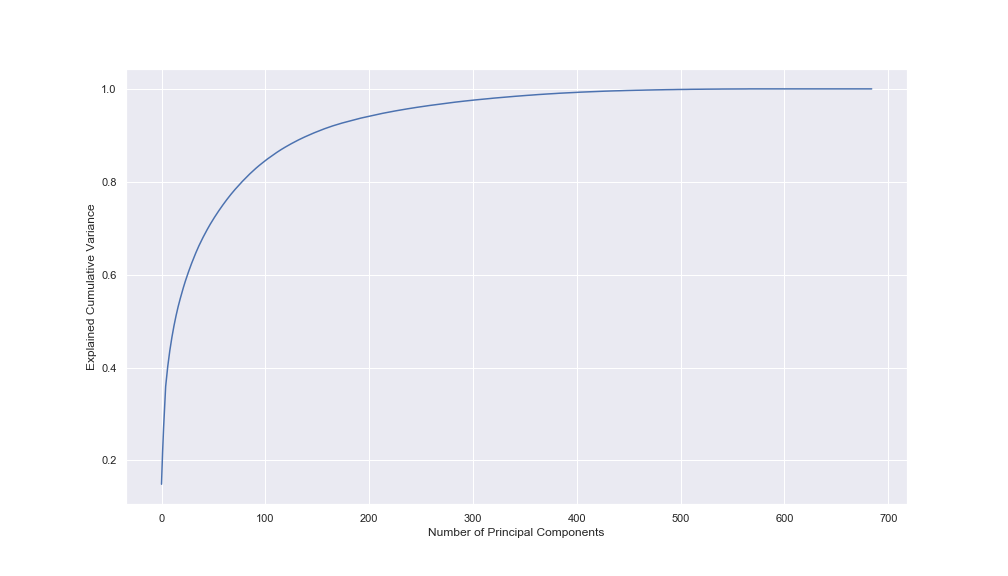
\includegraphics[width=0.8\textwidth, height=0.6\textwidth]{pca.png}
\caption{Principal Component Analysis}
\label{fig:pca}
\end{figure}

We check out the ratio of variance explained by each principal component as well as the cumulative variance explained. 

Based on the results from the PCA fitted previously, we decide to keep the first 150 reduced dimensions, that explain 90\% cumulative variance in data.

Now that we have our transformed principal components, we check out the weight of each variable on the first few components to see if we can interpret them some fashion.

Each principal component is a unit vector that points in the direction of highest variance (after accounting for the variance captured by earlier principal components). The further a weight is from zero, the more the principal component is in the direction of the corresponding feature. If two features have large weights of the same sign (both positive or both negative), then increases in one tend to expect to be associated with increases in the other. To contrast, features with different signs can be expected to show a negative correlation: increases in one variable should result in a decrease in the other.

To investigate the features, we map each weight to their corresponding feature name, then sort the features according to weight. The most interesting features for each principal component, are those at the beginning and end of the sorted list. 

We present here the investigation of feature associations from the first three principal components:

\begin{tabular}{lll}
    \textbf{Top 5 weights for PC1} \\
    D19\_GESAMT\_ONLINE\_QUOTE\_12 & 0.4903 & \multirow{5}{20em}{First component is all about online affinity and online transactions in the last 12 months} \\
    D19\_VERSAND\_ONLINE\_QUOTE\_12 & 0.4737 \\
    ONLINE\_AFFINITAET & 0.1393 \\
    D19\_BANKEN\_ONLINE\_QUOTE\_12 & 0.0913 \\
    D19\_GESAMT\_ANZ\_12 & 0.0885 \\
\end{tabular}

\begin{tabular}{lll}
    \textbf{Top 5 weights for PC2} \\
    ALTER\_HH & 0.3310 & \multirow{5}{25em}{Second component describes the number and age of inhabitants, affinity to religion, being traditional minded and money saver financial topology} \\
    SEMIO\_REL & 0.2465 \\
    SEMIO\_PFLICHT & 0.2112 \\
    FINANZ\_SPARER & 0.2055 \\
    ORTSGR\_KLS9 & 0.1711 \\
\end{tabular}

\begin{tabular}{lll}
    \textbf{Top 5 weights for PC3} \\
    ORTSGR\_KLS9 & 0.3036 & \multirow{5}{30em}{Third component describes the number and density per square kilometer of inhabitants, affinity to events and being sensual minded, as well as having the house as the main financial focus} \\
    EWDICHTE & 0.2092 \\
    SEMIO\_ERL & 0.1452 \\
    FINANZ\_HAUSBAUER & 0.1156 \\
    SEMIO\_LUST & 0.1153 \\
\end{tabular}

Next, we see how the data clusters in the principal components space. We apply k-means clustering to the dataset and use the average within-cluster distance to decide the number of clusters to keep. We use sklearn's KMeans class to perform k-means clustering on the PCA-transformed data.
 
We fit a KMeans model on the 150 reduced dimensions, and we investigate the change within-cluster distance across for a range of clusters between 2 and 16.

\begin{figure}[h]
\centering
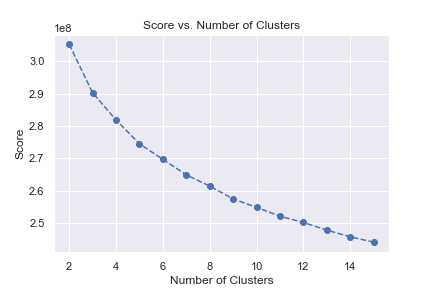
\includegraphics[width=0.8\textwidth]{images/kmeans.png}
\caption{Average within-cluster distances}
\label{fig:kmeans}
\end{figure}

Based on Figure \ref{fig:kmeans}, we can see that a good number of clusters is 8. We refit the k-means model with the selected number of clusters and obtain cluster predictions for the general population demographics data.

We compare the proportion of data in each cluster for the customer data to the proportion of data in each cluster for the general population:

\begin{figure}[h]
\centering
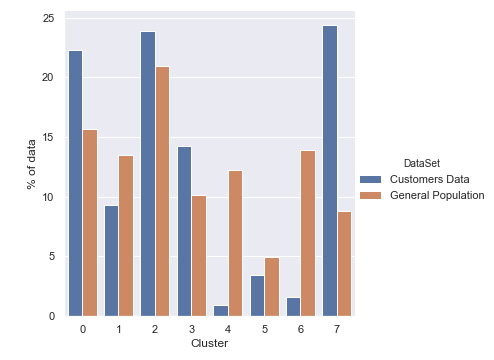
\includegraphics[width=0.8\textwidth, height=0.5\textwidth]{images/clusters.png}
\caption{Proportion of data points in each cluster for the general population and the customer data. }
\label{fig:clusters}
\end{figure}

We inspect what kind of people are part of a cluster that is over-represented in the customer data compared to the general population (cluster 7)

\begin{figure}[h]
\centering
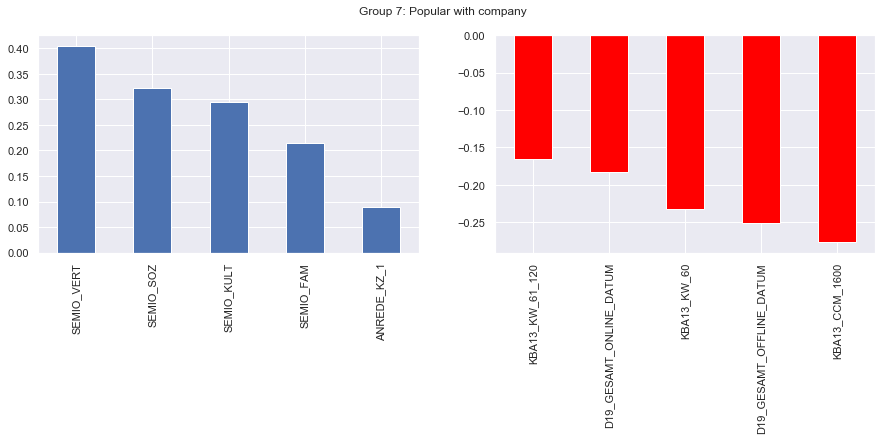
\includegraphics[width=0.8\textwidth, height=0.5\textwidth]{images/over_cluster.png}
\caption{Cluster 7 - People popular with the company }
\label{fig:overcluster}
\end{figure}

\paragraph{Popular with the company - Cluster 7} By using PCA's inverse transform we obtain the following values
\begin{itemize}
    \item SEMIO\_VERT (1) \# affinity indicating in what way the person is dreamily (highest affinity)
    \item SEMIO\_SOZ (2) \# affinity indicating in what way the person is social-minded (very high affinity)
    \item SEMIO\_KULT (3) \# affinity indicating in what way the person is cultural minded (high affinity)
    \item SEMIO\_FAM (6) \# affinity indicating in what way the person is familiar minded (very low affinity)
    \item ANREDE\_KZ\_1 (0) \# gender: female
\end{itemize}

We inspect what kind of people are part of a cluster with low representation in the customer data compared to the general population (cluster 4)

\begin{figure}[h]
\centering
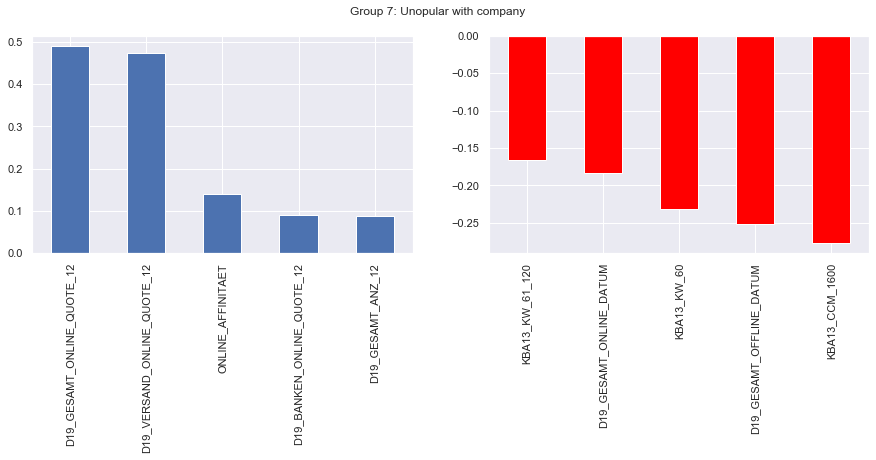
\includegraphics[width=0.8\textwidth, height=0.4\textwidth]{images/under_cluster.png}
\caption{Cluster 4 - People unpopular with the company }
\label{fig:undercluster}
\end{figure}

\paragraph{Unpopular with the company - Cluster 4} By using PCA's inverse transform we obtain the following values
\begin{itemize}
    \item D19\_GESAMT\_ONLINE\_QUOTE\_12 (0) \# amount of online transactions within all transactions in the complete file: no Online-transactions within the last 12 months
    \item D19\_VERSAND\_ONLINE\_QUOTE\_12 (0) \# amount of online transactions within all transactions in the segment mail-order: no Online-transactions within the last 12 months
    \item ONLINE\_AFFINITAET (2) \# online affinity: (average affinity)
    \item D19\_BANKEN\_ONLINE\_QUOTE\_12 (0) \# amount of online transactions within all transactions in the segment bank: no Online-transactions within the last 12 months
    \item D19\_GESAMT\_ANZ\_12 (1) \# transaction activity TOTAL POOL in the last 12 months: very low activity
\end{itemize}

\subsubsection{Supervised Learning Model}

To implement the supervised model, we start by preprocessing the training dataset using the same pipeline as above.

We use the unsupervised model fitted in the previous step to predict the cluster in which the observations are present.

We start by analysing the training dataset and especially the distribution between the two typs of responses: 0-non customer and 1-customer:

\begin{figure}[h]
\centering
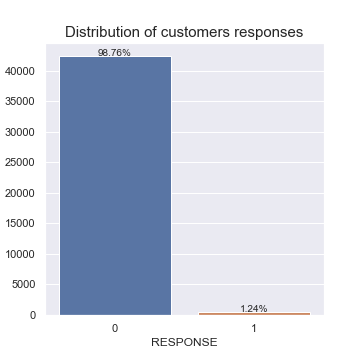
\includegraphics[width=0.8\textwidth]{images/customers_dist.png}
\caption{Distribution of customer responses shows that we are dealing with an imbalanced dataset}
\label{fig:cust_dist}
\end{figure}

There are several techniques to deal with an imbalanced dataset:
\begin{itemize}
    \item \textbf{Use the right evaluation metrics} - Evaluation metrics that can be applied in this case:
        \begin{itemize}
            \item Precision/Specificity: how many selected instances are relevant
            \item Recall/Sensitivity: how many relevant instances are selected
            \item F1 score: harmonic mean of precision and recall
            \item MCC: correlation coefficient between the observed and predicted binary classifications
            \item AUC: the relation between true-positive rate and false positive rate (\textbf{This is what we use in this project})
        \end{itemize}
    \item \textbf{Re-sample the training set} - Apart from using different evaluation criteria, one can also work on getting a different dataset. Two approaches to making a balanced dataset out of an imbalanced one are under-sampling and over-sampling.
        \begin{itemize}
            \item Under-sampling balances the dataset by reducing the size of the abundant class. This method is used when the quantity of data is sufficient. By keeping all samples in the rare class and randomly selecting an equal number of samples in the abundant class, a balanced new dataset can be retrieved for further modeling.
            \item Oversampling is used when the quantity of data is insufficient. It tries to balance dataset by increasing the size of rare samples. Rather than getting rid of abundant samples, new rare samples are generated by using, e.g., repetition, bootstrapping, or SMOTE (Synthetic Minority Over-Sampling Technique) \cite{SMOTE}.
        \end{itemize}
\end{itemize}

We split the dataset in train and test datasets by specifying that the two datasets are to be stratified using the target and keep the same weight for the classes. The proportion of data after splitting is 80\% for training and 20\% for validation.

We create a benchmark model using LogisticRegression with the default parameters, and then we fine-tune an XGBoostClasifier model using Bayesian optimization \cite{willkoehrsen2018}.

\subsection{Refinement}

We use several resampling techniques:
\begin{itemize}
    \item No resampling
    \item SMOTE -  Synthetic Minority Over-sampling Technique
    \item ADASYN - Adaptive Synthetic (ADASYN) sampling approach for imbalanced datasets
    \item ClusterCentroids - Method that under samples the majority class by replacing a cluster of majority samples by the cluster centroid of a KMeans algorithm. 
    \item TomekLinks -  Under-sampling by removing Tomek's links.
    \item SMOTETomek - Over-sampling using SMOTE and cleaning using Tomek links.
\end{itemize}

We also define a search hyperspace that we use to do a Bayesian parameter search. We define a search space for the following hyper-parameters for XGBoost:

\begin{itemize}
    \item 'n\_estimators': hp.quniform('n\_estimators', 100, 1000, 1),
    \item 'eta': hp.quniform('eta', 0.025, 0.5, 0.025),
    \item 'max\_depth':  hp.choice('max\_depth', np.arange(1, 14, dtype=int)),
    \item 'min\_child\_weight': hp.quniform('min\_child\_weight', 1, 6, 1),
    \item 'subsample': hp.quniform('subsample', 0.5, 1, 0.05),
    \item 'gamma': hp.quniform('gamma', 0.5, 1, 0.05),
    \item 'colsample\_bytree': hp.quniform('colsample\_bytree', 0.5, 1, 0.05),
    \item 'eval\_metric': 'auc',
    \item 'objective': 'binary:logistic',
    \item 'nthread': 4,
    \item 'booster': 'gbtree',
    \item 'tree\_method': 'gpu\_hist',
    \item 'silent': 1,
    \item 'seed': random\_state 
\end{itemize}